\subsection{Système d'aérofrein}

\subsubsection{Définition du système d'aérofreins}

Les besoins en termes de freinage aérodynamique sont relativement faibles. En effet, le but étant non pas de ralentir fortement la
fusée, mais simplement de créer un différencielle de trainée suffisamment importante entre les deux étages pour assurer une
séparation prpore. Sur-estimer cette trainée aurait pour conséquence d'augmenter fortement les efforts attendus sur la structure
des systèmes de séparation, et donc d'alourdir inutilement la fusée. De plus, une forte trainée pourrait engendrer une instabilité
de la fusée lors de la séparation des étages.\\

De ce fait, nous avons opté pour un système d'aérofreins de type "plaque déployable". Ce système est composé de deux bagues en
aluminium de 7 mm d'épaisseur et du même diamètre que l'intérieur du fuselage. Entre les deux plaques, un système de bielles permet
de déployer les aérofreins à l'aide d'un servo-moteur. Cela permet d'optenir un bon compromis entre la simplicité mécanique, le
poids et l'efficacité aérodynamique modérée.\\

\begin{minipage}{0.5\textwidth}
    \centering
    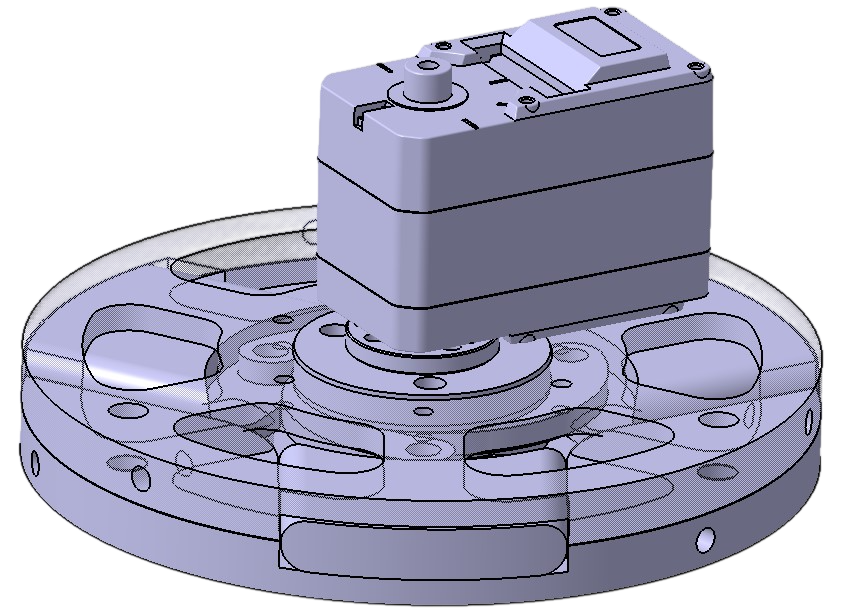
\includegraphics[width=\textwidth]{figures/Catia_AF_1.png}
    \captionof{figure}{Système d'aérofrein d'SP-02 sur \acrshort{CATIA}}
    \label{fig:aerofrein_SP02}
\end{minipage}
\hfill
\begin{minipage}{0.4\textwidth}
    Une vue du système d'aérofreins d'SP-02 est présentée à la figure \ref{fig:aerofrein_SP02}. Chaque bague est vissée au corps
    de la fusée par 4 vis M4, soit 8 vis M4 pour le système complet tout, réparties uniformément. Les deux bagues sont vissées
    entre elles par 3 vis M5. Cela permet de maximiser la rigidité du système et de transmettre les efforts aérodynamiques à la
    structure principale de la fusée. Les aérofreins à proprement parler sont constitués de plaques en \gls{POMc} de 7 mm
    d'épaisseur fixés entre les deux bagues à l'intéreur de rainures usinées dans chaque bague.
\end{minipage}

\begin{minipage}{0.34\textwidth}
    La figure \ref{fig:aerofrein_SP02_ouvert_ferme} montre les deux positions possibles des aérofreins. Le déploiement se fait à
    l'aide d'un servo-moteur placé à l'intérieur du fuselage et relié aux plaques par des bièles. Une rotation de 120° des plaques
    permet de passer de la position fermée à la position ouverte.
\end{minipage}
\hfill
\begin{minipage}{0.65\textwidth}
    \begin{figure}[H]
        \centering
        \begin{subfigure}{.49\textwidth}
            \centering
            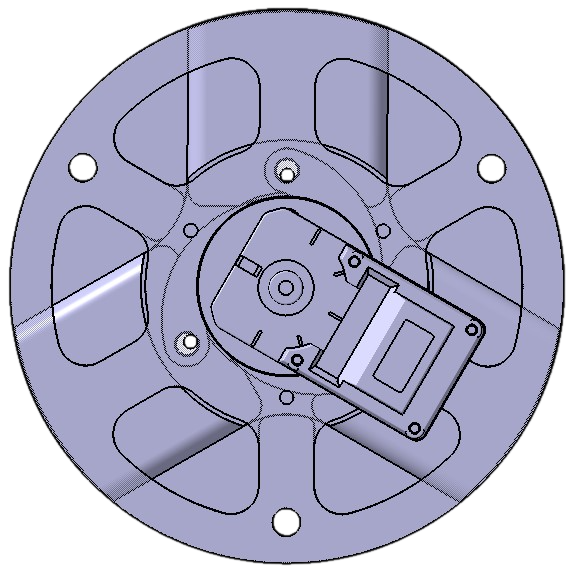
\includegraphics[width=0.75\textwidth]{figures/Catia_AF_2.png}
            \caption{fermé}
        \end{subfigure}
        \begin{subfigure}{.49\textwidth}
            \centering
            
\includegraphics[width=\textwidth]{figures/Catia_AF_3.png}
            \caption{ouvert}
        \end{subfigure}
        \caption{Position des aérofreins d'SP-02}
        \label{fig:aerofrein_SP02_ouvert_ferme}
    \end{figure}
\end{minipage}

\vfill

\begin{minipage}{0.55\textwidth}
    \centering
    \begin{tikzpicture}
        
        \node at (0, 0) {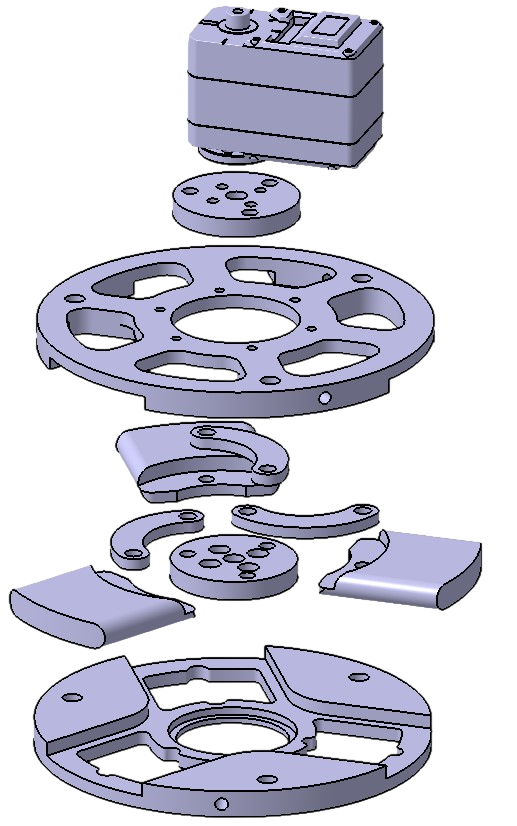
\includegraphics[width=0.8\textwidth]{figures/Catia_AF_4.png}};

        % \draw[help lines, step=1cm] (-3.5,-6) grid (6, 6);
        % \draw[help lines, step=0.5cm, lightgray] (-3.5,-6) grid (6, 6);
        % \draw[line width=2] (-3.5, +0.0) -- (+6.0, +0.0);
        % \draw[line width=2] (+0.0, -6.0) -- (+0.0, +6.0);

        \node (moteur_lbl)      at (+4.50, +4.50) {\textbf{Servo-moteur}};
        \node (rondelle1_lbl)   at (+4.50, +2.75) {\textbf{Rondelle 1}};
        \node (bague_haut_lbl)  at (+4.50, +1.75) {\textbf{Bague supérieure}};
        \node (rondelle2_lbl)   at (+4.50, +0.00) {\textbf{Rondelle 2}};
        \node (bielle_lbl)      at (+4.50, -1.00) {\textbf{Bielles (x3)}};
        \node (aerofrein_lbl)   at (+4.50, -2.00) {\textbf{Aérofreins (x3)}};
        \node (bague_bas_lbl)   at (+4.50, -4.00) {\textbf{Bague inférieure}};

        \draw [red, ->, line width=1.5] (moteur_lbl.west)     -- (+1.50, +4.50);
        \draw [red, ->, line width=1.5] (rondelle1_lbl.west)  -- (-0.25, +2.75);
        \draw [red, ->, line width=1.5] (bague_haut_lbl.west) -- (+1.50, +1.75);
        \draw [red, ->, line width=1.5] (rondelle2_lbl.west)  -- (+0.00, -1.25) -- (-0.25, -2.00);
        \draw [red, ->, line width=1.5] (bielle_lbl.west)     -- (+1.50, -1.50);
        \draw [red, ->, line width=1.5] (aerofrein_lbl.west)  -- (+2.00, -2.50);
        \draw [red, ->, line width=1.5] (bague_bas_lbl.west)  -- (+2.00, -4.00);

    \end{tikzpicture}
    \captionof{figure}{Vu éclatée du système d'aérofrein d'SP-02}
    \label{fig:aerofrein_SP02_eclate}
\end{minipage}
\hfill
\begin{minipage}{0.35\textwidth}
    La figure \ref{fig:aerofrein_SP02_eclate} présente une vue éclatée du système d'aérofrein. On y distingue les deux bagues
    en aluminium, les aérofreins en \gls{POMc}, les bielles de liaison en aluminium, les rondelles de maintien en \gls{POMc} et
    le servo-moteur. Le choix du matériau pour les aérofreins et les rondelles s'est porté sur le \gls{POMc} en raison de sa
    forte résistance mécanique, de sa facilité d'usinage et de son faible coefficient de frottement avec l'aluminium, ce qui
    réduit l'effort nécessaire pour le déploiement des aérofreins.\\

    La \acrshort{CAO} sur \acrshort{CATIA} nous indique une masse totale du système (servo-moteur inclus) de 360 g. Ce poids
    a été pris en compte dans la masse totale du premier étage tout comme dans le calcul de son centre de masse.\\
    
    La plus grande partie des pièces seront usinées au \gls{Skylab}. Seuls les aérofreins seront commandés à un fournisseur
    externe au vu de la complexité de leur forme nécessitant une fraiseuse 5 axes.\\

    L'ensemble des plans mécaniques du système d'aérofreins est disponible en annexe \ref{subsec:plan_aerofreins}.
\end{minipage}

\subsubsection{Modélisation de la cinématique des aérofreins}

La figure \ref{fig:cinematique_aerofrein} illustre la cinématique du système d'aérofreins.

\vfill

\begin{figure}[h!]
    \centering
    \begin{tikzpicture}
        \node at (0, 0) {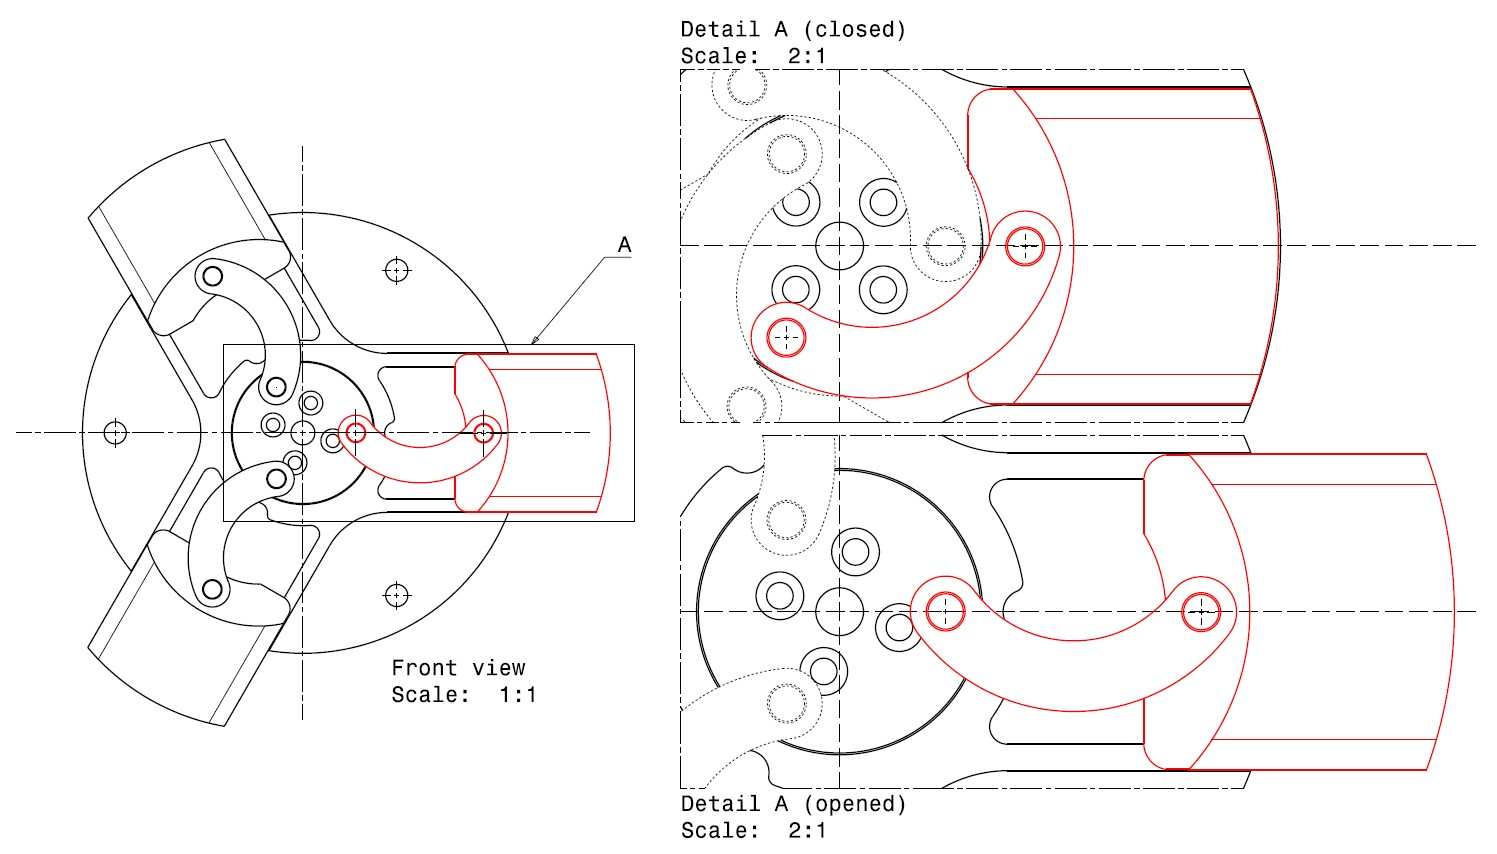
\includegraphics[width=\textwidth]{figures/Schema_AF.jpg}};

        % \draw[help lines, step=1cm] (-8, -4) grid (8, 4);
        % \draw[help lines, step=0.5cm, lightgray] (-8, -4) grid (8, 4);
        % \draw[line width=2] (-8.0, +0.0) -- (+8.0, +0.0);
        % \draw[line width=2] (+0.0, -4.0) -- (+0.0, +4.0);

        % Add half of transparency to the background image
        \filldraw[white, opacity=0.6] (-1, -4.8) rectangle (8, 4.8);

        \node (OA) at (1.03, 2.05) {};
        \node (OA_lbl) at (1.25, 2.25) {\textbf{O}};

        \node (AA) at (0.42, 1.00) {};
        \node (AA_lbl) at (0.25, 0.75) {\textbf{A}};

        \node (BA) at (3.15, 2.05) {};
        \node (BA_lbl) at (3.25, 2.25) {\textbf{B}};

        \draw[circle, dotted, line width=1.5] (OA) circle (1.2143);

        \draw[line width=1.5, red, <->] (OA.center) -- (AA.center) node [midway, above left] {\textbf{R}};
        \draw[line width=1.5, blue, <->] (AA.center) -- (BA.center) node [midway, below] {\textbf{L}};

        \draw (1.4, 2.05) arc (0:-120:0.3cm) node [midway, right] {\textbf{$\theta$}};


        \node (OB) at (1.05, -2.1) {};
        \node (OB_lbl) at (0.75, -1.75) {\textbf{O}};

        \node (AB) at (2.26, -2.1) {};
        \node (AB_lbl) at (2.5, -1.5) {\textbf{A}};

        \node (BB) at (5.15, -2.1) {};
        \node (BB_lbl) at (5.3, -1.75) {\textbf{B}};

        \draw[circle, dotted, line width=1.5] (OB) circle (1.2143);

        \draw[line width=1.5, red, <->] (OB.center) -- (AB.center) node [midway, below] {\textbf{R}};
        \draw[line width=1.5, blue, <->] (AB.center) -- (BB.center) node [midway, below] {\textbf{L}};

        \draw[line width=1.5, <->] (5.75, -4.1) -- (7.75, -4.1) node [midway, below] {\textbf{D}};


        % Add i, j units vectors
        \draw[->, line width=1.5] (-1.0, -3.5) -- (-0.0, -3.5) node [midway, above] {\textbf{i}};
        \draw[->, line width=1.5] (-1.0, -3.5) -- (-1.0, -2.5) node [midway, left] {\textbf{j}};

    \end{tikzpicture}
    \caption{Schéma de la cinématique des aérofreins}
    \label{fig:cinematique_aerofrein}
\end{figure}

\vfill

La cinématique du système d'aérofreins est définie par trois paramètres principaux : la longueur caractéristique des bielles
($AB = L$), la distance entre l'axe de rotation des aérofreins et le point de fixation des bielles ($OA = R$), et l'angle de
rotation de ce point ($\widehat{AOB}=\theta$).\\

D'après la formule d'Al Kashi, on peut exprimer la distance $OB$ en fonction de ces paramètres :
\begin{align}
    AB^2    &= OA^2 + OB^2 - 2 \cdot OA \cdot OB \cdot \cos(\theta) \\
    L^2     &= R^2 + OB^2 - 2 R \cdot OB \cdot \cos(\theta) \\
    0       &= OB^2 - 2 R \cos(\theta) \cdot OB + (R^2 - L^2) \\
    OB      &= \frac{2 R \cos(\theta) \pm \sqrt{(2 R \cos(\theta))^2 - 4 (R^2 - L^2)}}{2} \\
            &= R \cos(\theta) \pm \sqrt{R^2 \cos^2(\theta) - (R^2 - L^2)} \\
            &= R \cos(\theta) \pm \sqrt{L^2 - R^2 \sin^2(\theta)}
\end{align}

Pour le cas $OB = R \cos(\theta) - \sqrt{L^2 - R^2 \sin^2(\theta)}$, on remarque que:
\begin{align}
    0 &\leq OB\\
    0 &\leq R \cos(\theta) - \sqrt{L^2 - R^2 \sin^2(\theta)}\\
    \sqrt{L^2 - R^2 \sin^2(\theta)} &\leq R \cos(\theta) \\
    L^2 - R^2 \sin^2(\theta) &\leq R^2 \cos^2(\theta) \\
    L^2 &\leq R^2 (\sin^2(\theta) + \cos^2(\theta)) \\
    L^2 &\leq R^2 \\
    L &\leq R
\end{align}

Or, dans notre cas, $L > R$. Nous rejetons donc cette solution et retenons :

\begin{equation}
    OB = R \cos(\theta) + \sqrt{L^2 - R^2 \sin^2(\theta)}
\end{equation}

La distance $D$ est donnée par la différence entre $OB$ et le rayon de l'extérieur de la fusée $R_{fusee}$ :

\begin{equation}
    D(\theta) = R \cos(\theta) + \sqrt{L^2 - R^2 \sin^2(\theta)} - R_{fusee}
\end{equation}

La surface projetée $S$ des aérofreins peut être approchée par la surface d'un rectangle de largeur $D$ et de hauteur $H$ (hauteur
des aérofreins) multipliée par le nombre d'aérofreins (3) :

\begin{align}
    S(\theta) &= 3 \cdot H \cdot D(\theta) \\
    \Aboxed{S(\theta) &= 3 \cdot H \cdot \left( R \cos(\theta) + \sqrt{L^2 - R^2 \sin^2(\theta)} - R_{fusee} \right)} \label{eq:surface_aerofrein}
\end{align}

La formule \ref{eq:surface_aerofrein} pourra être utilisée dans les calculs aérodynamiques pour estimer la trainée générée par les
aérofreins en fonction de leur angle de déploiement $\theta$.

\newpage